% LaTeX file for resume 
% This file uses the resume document class (res.cls)

\documentclass[margin]{res}
\usepackage{graphicx}

\usepackage{wrapfig}

%\usepackage{helvetica} % uses helvetica postscript font (download helvetica.sty)
%\usepackage{newcent}   % uses new century schoolbook postscript font  
\topmargin=-0.5in  % start text higher on the page
\setlength{\textheight}{10in} % increase text height to fit resume on 1 page
\begin{document}
	
	\newcommand{\cba}[2]{
		\bf\hspace{.08in}#1\normalfont
		\begin{itemize}
			\item[] #2\\
		\end{itemize}
		}
		
	\newcommand{\cbb}[3]{
		\begin{tabular}{p{2.5in} r}
			{\bf #1}, &  #2
		\end{tabular}	
		\begin{itemize}
			\item[] #3 
		\end{itemize}}
	
	\name{Cihan Sari}
	
	\address{Bordenbergweg Str. 64367, M\"uhltal\\
		\hspace{.5in}+49 176 62 01 37 66\\
		\hspace{.55in}csari@cihansari.com}
	%\begin{figure}[h!]
	%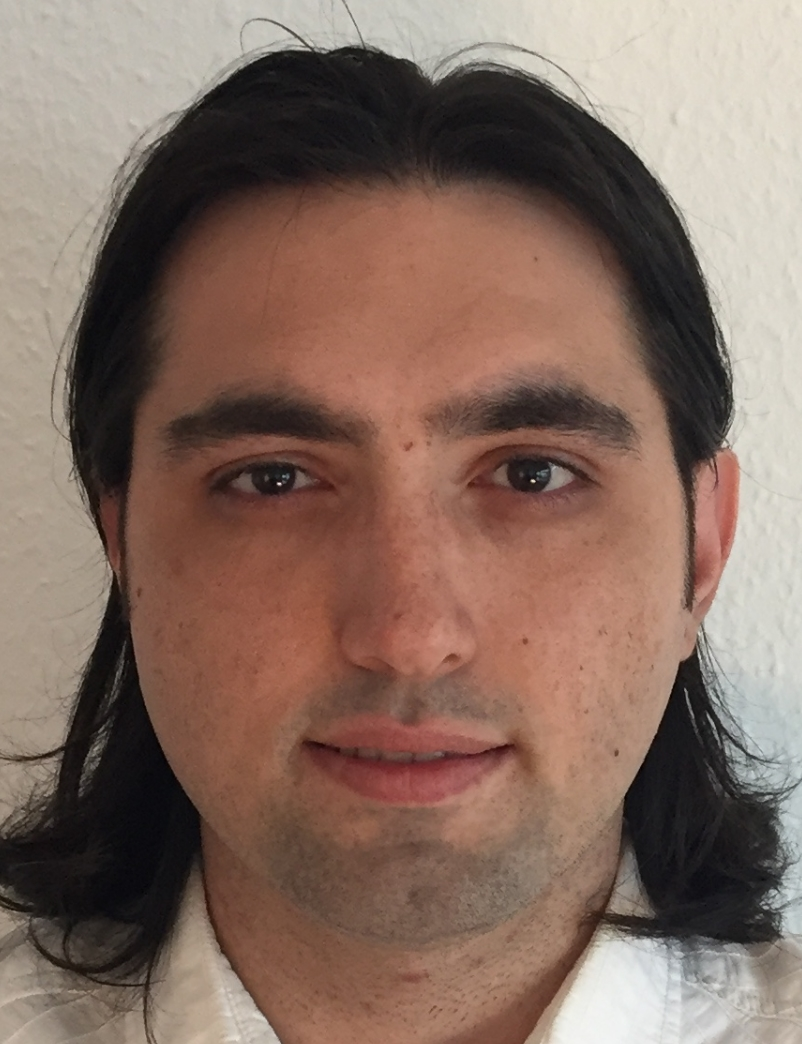
\includegraphics{me.jpg}       
	%              \end{figure}          d
	\begin{resume}
		\begin{wrapfigure}{r}{0.1\textwidth}
			\vspace{-1in}
			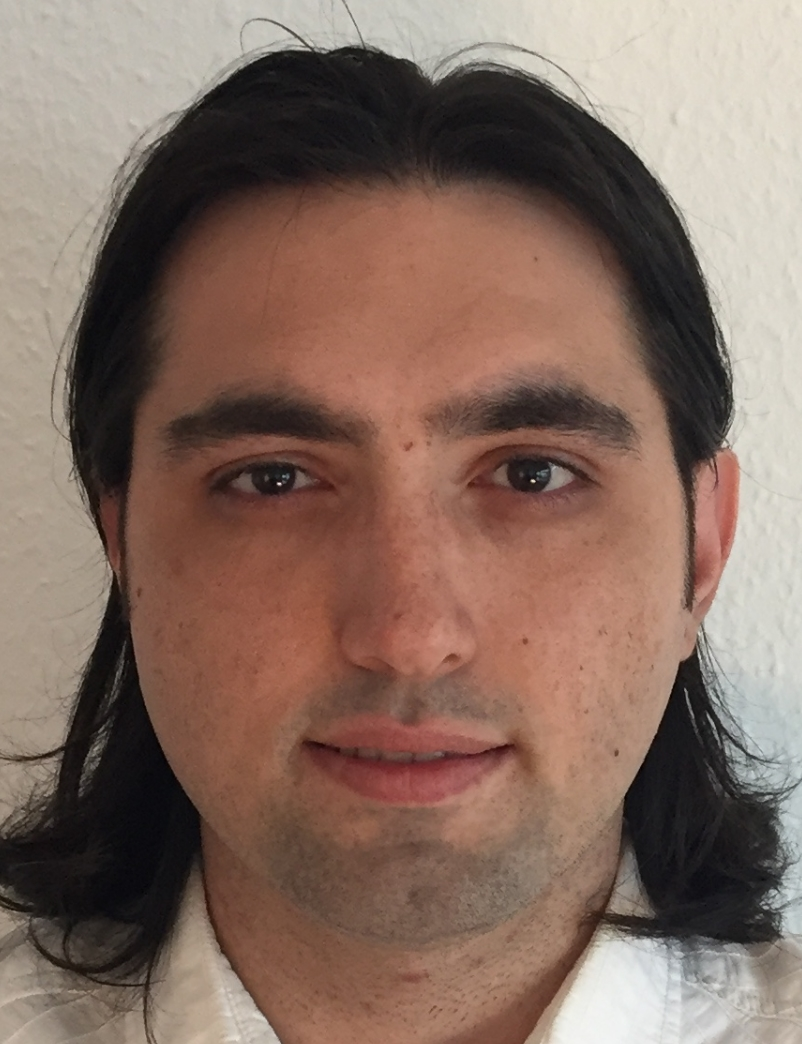
\includegraphics[width=1in]{me.jpg}
		\end{wrapfigure}
		
		\vspace{.5in}
		\section{SKILLS}
		\cba{Programming}{C++, Qt, C\#, Matlab, Bash}
		\cba{Subjects of Interest}{Machine Learning, Pattern Recognition, Computer Vision}
		\cba{Personal}{Team player, Hard worker, and Researcher}
		
		\vspace{.5in}

		\section{EXPERIENCE}
		\cbb{ISRA Vision AG}{January 2016 - (currently ongoing)}
		{R\&D Project Manager on Corporate \& Electronics, Illuminations and Sensors center, sensor and hardware solutions, development and management}
		
		\cbb{Vistek ISRA Vision}{January 2014 - December 2015 (2 years)}
		{R\&D Manager of research and development team of machine vision based solutions for industrial automation and inspection as well as computer vision applications}
		
		\cbb{Bo\u{g}azi\c{c}i Uni. Signal and Image Processing Laboratory}{February 2012 -  December 2013}
		{Member of research team}
		
		\cbb{Vistek ISRA Vision}{February 2010 - October 2013 (3 years 9 months)}
		{Member of research and development team of machine vision based solutions for industrial automation and inspection as well as computer vision applications}
		
		\vspace{.5in}
		\section{EDUCATION}
		\cbb{Bo\u{g}azi\c{c}i University}{Istanbul}
		{Systems and Control Engineering (MSc) - ongoing\\G.P.A. 3.6/4.0}

		\hspace{.08in}{\bf Subjects}\vspace{-.15in}\\
		\begin{itemize}
			\item[] Introduction to Image Processing \\
			Introduction to Robot Control\\
			Pattern Recognition \\
			Computer Vision \\
			Data Mining for Visual Media \\
			Autonomous Robots \\
			Optimization Techniques \\
			Stochastic Processes \& Applications
		\end{itemize}
		
		\cbb{Yeditepe University}{Istanbul}
		{Electrical and Electronics Engineering (BSc), 2010\\G.P.A. 2.6/4.0}

		\hspace{.08in}{\bf Subjects}\vspace{-.15in}\\
		\begin{itemize}
			\item[] Digital Signal Processing \\
			Digital Control \\
			Micro Controllers
		\end{itemize}

		\section{PROJECTS}
		\section{ISRA Vision Projects}
		\cbb{BeadMaster}{2016 - ongoing}{Glass cup quality inspection machine (mouth, sides, surface, brim and bottom purity inspection). Worked on vision solutions for mouth, sides and surface purity inspection and as coordinator between vision and software team.}
		\cbb{TIS}{2014 - 2015}{Tumbler Inspection System, quality inspection machine (mouth, sides, surface, brim and bottom purity inspection). Worked as team manager development for mouth, sides and surface purity inspection and as coordinator between vision and software team.}
		\cbb{TIS}{2011 - 2013}{Tumbler Inspection System, quality inspection machine (mouth, sides, surface, brim and bottom purity inspection). Worked on vision solutions for mouth, sides and surface purity inspection and as coordinator between vision and software team.}
		\cbb{Torpedo Inspection}{2013}{Worked on core program, vision algorithm, user interface and database.}
		\cbb{Color Inspection}{2013}{Worked on core program, user interface, database and machine vision. Color inspection is used for both biscuits and fabrics.}
		\cbb{Refrigerator Measurement System}{2012}{Worked on vision algorithm, detection of interest point in the images, calibrating 10 cameras to work in the same workspace.}
		\cbb{Texture Matching}{2011}{Worked on fabric texture matching using Scale Invariant Feature Transform (SIFT), Sped up Robust Features (SURF) and bag of visual words (BoW).}
		\cbb{VisMos}{March - June 2010}{Granite / Marble Mosaic Tile Setting System. Worked on accurate tile position and color detection to provide exact coordinates for robot arm to pick up the tiles.}

		\section{In Proceedings}

		\begin{itemize}
			\item[] \underline{C. Sari}, C. B. Akgul, B. Sankur.Combination of Gross Shape Features, Fourier Descriptors and Multiscale Distance Matrix for Leaf Recognition. In 55th International Symposium ELMAR-2013, Zadar, Croatia, September 25-27, 2013. 
		\end{itemize}	

		\begin{itemize}
			\item[] G. Kayim, \underline{C. Sari}, Ceyhun Burak Akgul.Facial Feature Selection for Gender Recognition based on Random Decision Forests. In 21. Sinyal {\.I}\c{s}leme ve {\.I}leti\c{s}im Uygulamalar{\i} Kurultay{\i} (SIU-2013), Girne, Kuzey K{\i}br{\i}s T\"{u}rk Cumhuriyeti, 24-25 Nisan, 2013.
		\end{itemize}
		
		
		\section{Grad and Personal Projects}
			\cbb{Gender Data for Face Images}{2015}{Hobala hobala hobalafdaisfjdasfkasfja jfdkas f dksfjdas ldjas fdlasdjkls fdlaskfdas mm dasmdafkdasfdkasfaiasd jdais jsdias fjdasfh dasfjas hdjas hfdjashfdas fjhdasfu dhasfua.}
			
			\cbb{Style Transfer}{2015}{Hobala hobala hobalafdaisfjdasfkasfja jfdkas f dksfjdas ldjas fdlasdjkls fdlaskfdas mm dasmdafkdasfdkasfaiasd jdais jsdias fjdasfh dasfjas hdjas hfdjashfdas fjhdasfu dhasfua.}
			
			\cbb{Database Sorter}{2015}{Hobala hobala hobalafdaisfjdasfkasfja jfdkas f dksfjdas ldjas fdlasdjkls fdlaskfdas mm dasmdafkdasfdkasfaiasd jdais jsdias fjdasfh dasfjas hdjas hfdjashfdas fjhdasfu dhasfua.}
			
			\cbb{Hough Forests based Face Detection}{March - April 2012}{Project for Data Mining for Visual Media course, Hough Forests architecture is investigated for face detection using OpenCV 2.4.3, Qt 5.0.1. 3000 samples from cropped labeled faces in the wild (LFW) dataset is used for training decision forests. Faces are divided to 16 patches ($4\times4$). Extremely randomized trees are given an objective to classify the face patches. A tiny program is used to generate these trees using a part of the training set and this program is distributed to 14 computers. Each computer generated $500 - 1200$ unique trees and according to their individual and combined performances, each has reached to the generalized error that is proposed by RDF ($40\%$ accuracy on identifying a patch correctly). Finally, probabilistic voting is used to determine the face in the image. 99.37\% performance is reached on Cropped LFW (on remaining 10233 test images) and 70.60\% on 13233 full LFW images.}
				
			\cbb{Random Decision Forests}{April 2012}{As part of the Data Mining for Visual Media course, a two hours RDF presentation is given to the class, including decision trees, studies that lead to RDF, its algorithm, parameters and advantages, some tricks on its usage, comparisons against SVM and Neural Networks and popular studies.}
			
			\cbb{Home Service Robot}{April 2012}{Project for Autonomous Robots course using Robot Operating System (ROS), Qt 4.6.4, OpenCV 2.4.2. 10 minutes are given to simultaneously map the environment and position the robot. Afterwards, random requests are given to the robot via control panel to go to drink, where robot requests it, then goes to the visitor. Robot gives requests using speech synthesis module and takes requests using speech recognition. Environment is simulated using Virtual Robot Experimentation Platform (V-Rep), a control panel to handle requests, keep track of the current map, robot position, emergency stop etc. is coded using Qt. Same interface can be used to manually move robot in the map or katana arm (although obstacle avoidance module overrides this control when necessary). OpenCV is used to create the map, visualize it, identify objects of the surrounding (drink, user, door handles). Orocos Kinematics Dynamics (KDL) package is used for arm dynamics to open the doors using robot arm. Rapidly exploring random trees (RRT) is implemented for path finding.}	           	
			
			\cbb{Leaf Recognition}{October - December 2011}{Project for Introduction to Image Processing and Computer Vision course, which eventually lead to "Combination of Gross Shape Features, Fourier Descriptors and Multiscale Distance Matrix for Leaf Recognition" study. It recognizes the provided leaves using three separate SVM classifiers trained with respective feature sets and determines the final decision by weighing decisions with cross-validation performances.}
			
			\cbb{Gender Recognition with Random Decision Forests}{October - December 2011}{Project for Pattern Recognition course, which eventually lead to a joint study "Facial Feature Selection for Gender Recognition based on Random Decision Forests". Throughout the tests, the number of necessary features that is used on SVM is successfully reduced to half (445 features out of total 832) with 1.4\% performance sacrifice.}
			
	
	\end{resume} 
\end{document}